\chapter{ABC}

This chapter will outline a series of illustrative ABC examples. These will serve to demonstrate core concepts touched on in the introduction, demonstrate ABC can sample from complex distributions, and develop the boutique code base which form the foundations of this project. The code for the examples in this section can be found at \url{https://github.com/tomconnell/dram}.\\

\section{Toy problem 1: 1D Gaussian}
As a simple first example consider we have observed $n = 100$ realizations from the Gaussian model $\bm{g_s}(\bm{\theta}) = \frac{1}{\sqrt{2\pi\sigma^2}}\ \text{exp}\Big[\frac{-\mu^2}{2\sigma^2}\Big]$. Our unknown model parameters are $\bm{\theta} = [\mu,\sigma]$. Given we have access to simulation from this model it is possible to leverage ABC algorithms to estimate these unknown model parameters. A synthetic dataset for this problem is created with $\mu = 5$ and $\sigma = 2$. The summary statistics sample mean, $\bar{\mu}$, and sample standard deviation, $\bar{\sigma}$, are used. These provide sufficient statistics with a 1:1 correspondance to the unknown parameters. Figure \ref{toy1-fig1} plots the ABC posterior obtained from using algorithm \ref{ABCrejectionsampler}, the traditional form of an ABC rejection sampler, compared to the analytical likelihood. The metric over summary statistics is evaluated marginally and hence takes the form $\text{d}(\bm{S}(\bm{y}),\bm{S}(\bm{y^*})) = |S_1(\bm{y^*}) - S_1(\bm{y})| +| S_2(\bm{y^*}) - S_2(\bm{y})|$. A uniform prior is used to give equal probability to a bounded area, $p(\mu) = \mathcal{U}(0,10)$ and $p(\sigma) = \mathcal{U}(0,10)$. 
Figure \ref{toy1-fig2} explores the impact of varying the tolerance for this problem.\\

\begin{figure}[H]
	\centering
	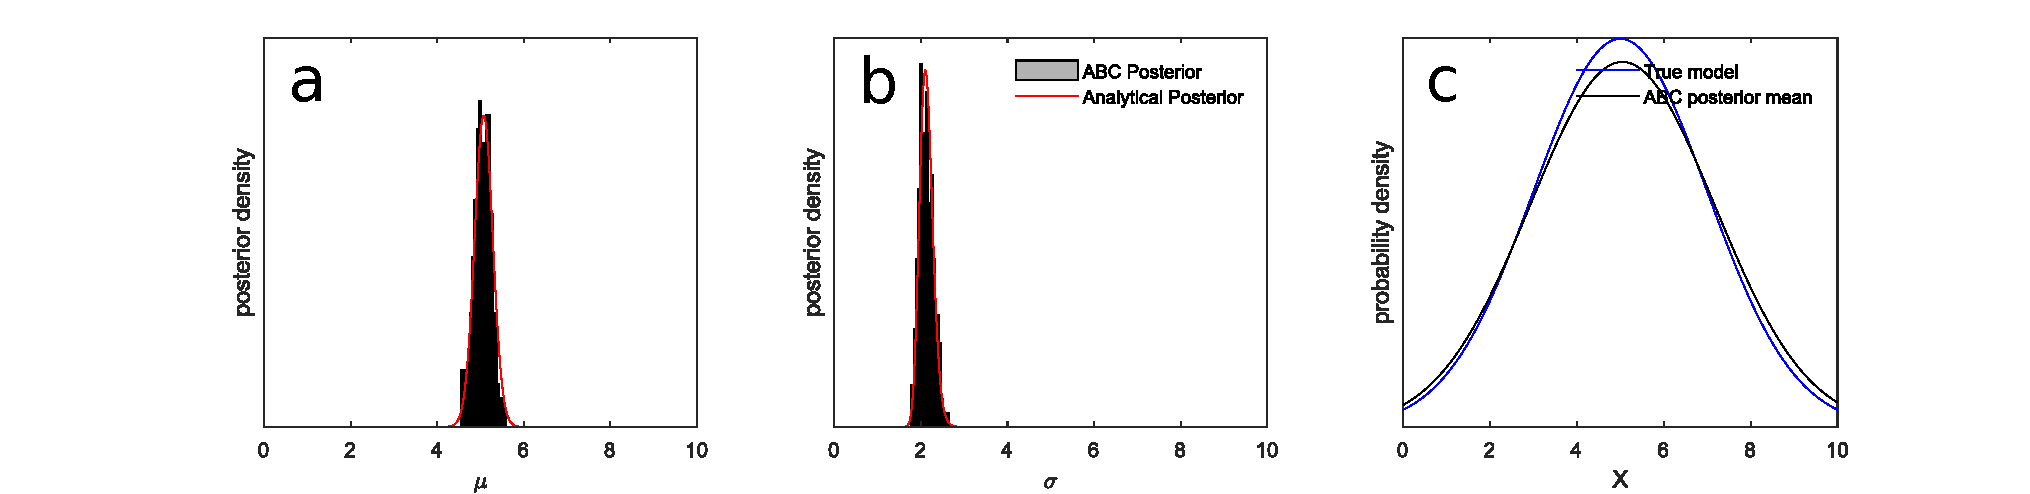
\includegraphics[scale=0.45]{toy1-fig1.pdf}
	\caption{Posterior comparison between ABC and traditional likelihood inference for estimating the parameters, $\bm{\theta} = [\mu,\sigma]$, to a Gaussian model given $n = 100$ observations, $\bm{y}$. The ABC algorithm, algorithm \ref{ABCrejectionsampler}, uses 1 million repititions and a tolerance $\epsilon = 0.1$. The likelihood takes the form $\mathcal{L}(\bm{\theta}|\bm{Y}) = (2\pi\sigma^2)^{-n/2}\ \text{exp}\big[-\frac{1}{2\sigma^2}\sum_{i = 1}^{n}(y_i-\mu)^2\big]$. (a) Marginal posterior compared to marginal ABC posterior for unknown parameter $\mu$. (b) same as (a) but for unknown parameter $\sigma$. (c) Mean ABC posterior model compared to true model.}
	\label{toy1-fig1}
\end{figure}

\begin{figure}[H]
	\centering
	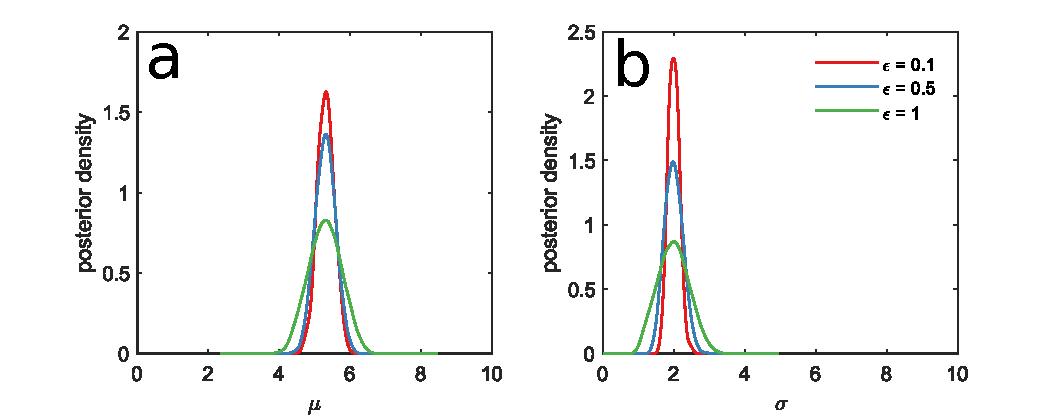
\includegraphics[scale=0.6]{toy1-fig2.pdf}
	\caption{The effect of varying the tolerance $\epsilon$ when estimating $\bm{\theta} = [\mu,\sigma]$ to a Gaussian model given given $n = 100$ observations, $\bm{y}$. Three tolerances are considered, $\epsilon = 0.1$, $\epsilon = 0.5$, $\epsilon = 1$. (a) Marginal ABC posterior for unknown parameter $\mu$. The true value is $\mu = 5$ (b) same as (a) but for unknown parameter $\sigma$. The true value is $\sigma = 2$}.
	\label{toy1-fig2}
\end{figure}

Figure \ref{toy1-fig1} demonstrates that with sufficient statistics and a low tolerance ABC can accurately resolve the posterior using only the ability to simulate data. However, as figure \ref{toy1-fig2} demonstrates, high tolerances erode posterior accuracy and uncertainty is over-estimated. However, it is true that increasing the tolerance increases the acceptance rate and hence relaxes computational resources. In this case the acceptance rate with $\epsilon = 0.1$ was $0.021\%$, while the acceptance rate with $\epsilon = 1$ was $2.023\%$. Under a model which is expensive to simulate from, walking the tightrope between accuracy and efficiency becomes important and needs to be carefully examined. In spite of shortcomings, the strengths of the ABC rejection sampler has led to significant scientific experiments \citep{Fu1997,Weiss1998a,Pritchard1999a}.

\section{Toy problem 2: Linear regression}
\label{sec-lin-reg}

As a second example consider we have observed some data, $\bm{y}$, from the linear model $\bm{g}(\bm{\theta}) = m\bm{x} + b$ and there is some stochasticity in the measurement process such that $\bm{g_s}(\bm{\theta}) = \bm{g}(\bm{\theta}) + \mathcal{N}(0,\sigma^2)$. Our unknown parameters are $\bm{\theta} = [m,b]$, while $\sigma$ is known. In this case it is deemed that computational resources are limitied and MCMC, which uses local transitions, will be needed to improve acceptance rates. MCMC will also be needed when the search spaces are high dimensional, with many unknown parameters, or the posterior is a long way from the prior. For this case we can call upon ABC-MCMC in the form of algorithm \ref{ABC-MCMC}. \\

Algorithm \ref{ABC-MCMC} samples the ABC posterior, equation \ref{summary-stat-abc-posterior}. The algorithm relies on evaluating the M-H acceptance probability, equation \ref{M-H-acce}. In our implementations Gaussian transition kernels, $q(.,.)$, are strictly used. As such the transition kernels cancel out in equation \ref{M-H-acce}. That leaves the prior and the weighting kernel to be evalutated at each time step in the Markov chain. The weighting kernel takes the form of equation \ref{generic-weighting-kernel}. In this case a uniform weighting kernel, $K_U$, is implemented. The interpretation of $K_U$ is the same as the accept/reject step in the rejection sampler: 
\begin{equation}
	K_U = 
	\begin{cases}
		1 & \text{if}\ 	\frac{\text{d}(S_i(\bm{y^*}),S_i(\bm{y}))}				{\epsilon_i} \leq 1\\
		0 & \text{if}\ \frac{\text{d}(S_i(\bm{y^*}) - S_i(\bm{y}))}				{\epsilon_i} > 1
	\end{cases}
\end{equation}
$K_U$ hence forms an indicator function $\mathbbm{1}$ which is equal to $1$ when the distance between statistics, which are fit marginally, is less than the tolerance. Given, $\bm{S} = \{S_1,\dots,S_O\}$, the weighting kernel takes the form:
\begin{equation}
	p(\bm{S}(\bm{y})|\bm{S}(\bm{y^*}),\bm{\theta}) = \prod_{i = 1}^{O} K_U\Big(\frac{\text{d}(S_i(\bm{y}),S_i(\bm{y^*})}{\epsilon_i}\Big)
	\label{weight-kernel}
\end{equation}
\noindent
As with the 1D Gaussian example it would be possible to take summaries which have a 1:1 correspondance to the unknown parameters. For a given simulation, a linear model could be fit to the simulated data. The slope and intercept of the fit model could then be used as summaries. However, to demonstrate that this is not necessary, we take inspiration from \citet{vrugt2013toward} and use sample mean, $\bar{\mu}$, and sample standard deviation, $\bar{\sigma}$, as summary statistics. The slope is restricted to a positive value to make these statistics sufficient. \\

Figure \ref{linear-regression} shows ABC-MCMC applied to the linear regression problem. \\

In the next section we continue to introduce algorithmic considerations into ABC as we build toward a geophysically relevant parameter estimation system. \\

\begin{figure}[H]
	\centering
	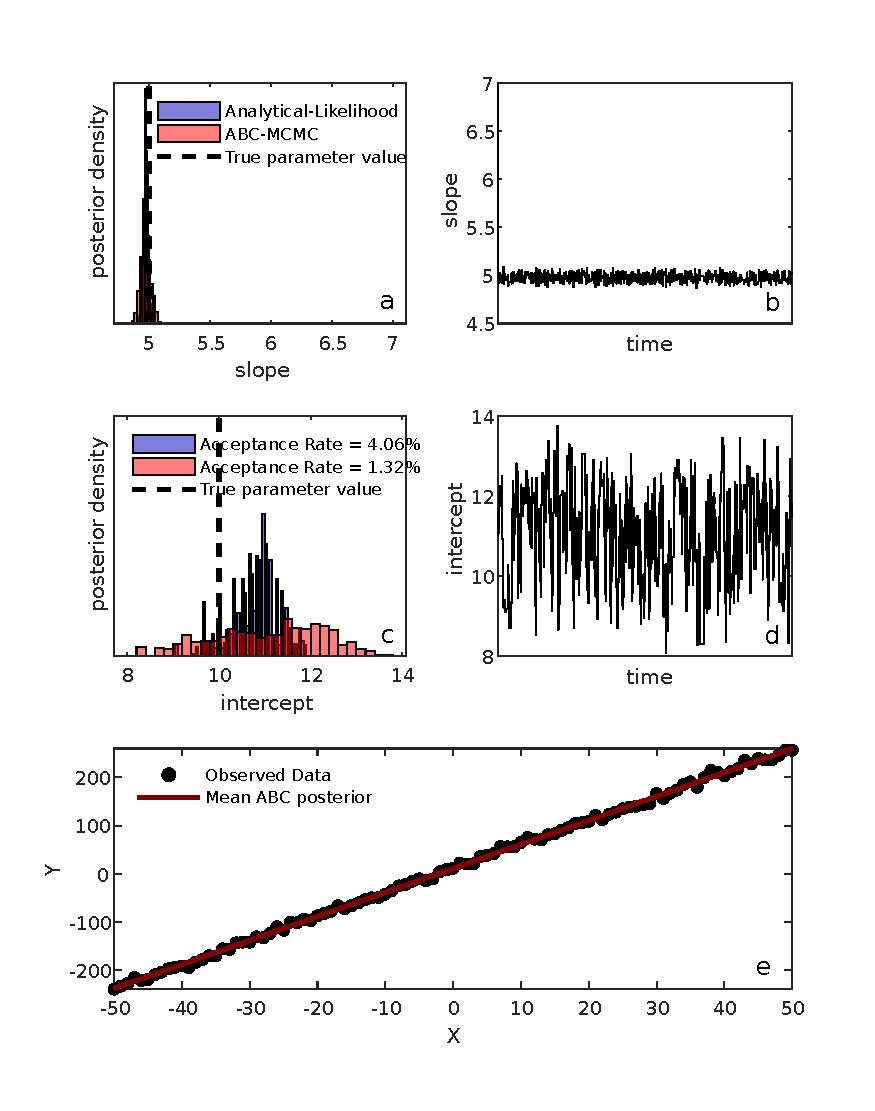
\includegraphics[scale=1.1]{linear-regression-example.pdf}
	\caption{Linear regression with ABC. The ABC posterior is also compared to traditional likelihood machinary. MCMC is used to sample both posteriors. For ABC tolerance is $\bm{\epsilon} = [2,2]$. For both the transition kernel is $q = \mathcal{N}([0,0],I)$. The Markov chain length is $20\ 000$. (a) The marginal ABC posterior and marginal analytical posterior compared for unknown parameter $m$. (b) Plot of the ABC-MCMC Markov chain through time for $m$. (c) Same as (a) except for unknown parameter $b$. (d) Same as (b) except for unknown parameter $b$. (e) Comparison of the mean ABC posterior model and the observed data generated with $m = 5$, $b = 10$ and $\sigma = 5$.}
	\label{linear-regression}
\end{figure}

%This example truly highlights how ABC shifts away from many traditional %Bayesian and frequentist techniques which rely computing data residuals in the %form $\sum (\bm{g}(\bm{\theta})-\bm{y})^2$. This residual is computed in the %analytical linear regression likelihood and is at the heart of all likelihood %functions which are applied in geophysics, equation \ref{likelihood-1} and %equation \ref{likelihood-2}. Instead, ABC opts for informal measures of %'goodness-of-fit' and rely on user-varied tolerances, which guarentee %posteriors close to the true posterior, save for a small degree of bias. The %result of a tolerance $> 0$ and summary statistics which do not always measure %fitness as tightly as a data residual. However the gain is in diagnostic %power. The data residual takes all the information in the data set and mixes %it into a single number, the residual value. However, the form of ABC allows %for the state of the algorithm at any one stage to be evaluated and fitting %statistics marginally means different rules can be set for different %statistics depending on what they mean to the inversion. Understanding how %statistics change through an inversion, the nature in which they diverge, and %the degree to which they spread around the observed value has taught %researches in other disciplines a great deal about the nature of their models %and the systems in which they study. That same central idea should be %transferrable to geophysical parameter estimation problems and may offer room %for more diagnostic inversion schemes, one with a greater deal of user control %and greated deal of interprebable meaning. \\

\section{Toy problem 3: Bivariate Gaussian}
% Introduce the problem
As a third example consider we $n = 100$ observations from a bivariate Gaussian distribution $\mathcal{N}(\bm{\mu},\bm{\Sigma})$ with $\bm{\mu} = \begin{bmatrix}
\mu_X\ \mu_Y
\end{bmatrix}^T$ and $\bm{\Sigma} = \begin{bmatrix}
\sigma^2_X & \rho\sigma_X\sigma_Y\\
\rho\sigma_X\sigma_Y & \sigma^2_Y
\end{bmatrix} $ where both $\bm{\mu}$ and $\bm{\sigma}$ are unknown, hence $\bm{\theta} = [\bm{\mu},\bm{\Sigma}]$. Figure \ref{init-qualms}(a) shows the observed data and the underlying causitive distribution. This example has 5 unknown parameters in total and as such we can appeal to ABC-MCMC for efficient sampling. The weighting kernel takes the same form as equation \ref{weight-kernel} and summaries with a 1:1 correspondance to the unknown parameters are used, the marginal sample means, $\bar{\mu_X}$ and $\bar{\mu_Y}$, standard deviations, $\bar{\sigma_X}$ and $\bar{\sigma_Y}$, and sample covariance, $\text{cov}(X,Y)$. The prior distribution, $p(\bm{\theta}) = \mathcal{U}(0,10)$, is used to provide equal probability to a bounded area for all unknowns beside correlation, $\rho$, which bounded as $p(\rho) = \mathcal{U}(-1,1)$. Figure \ref{init-qualms}(b) shows the results of the first 10 000 time steps from an ABC-MCMC. It can be seen that the algorithm is stationary for the first 3 000 repititions.\\

%% Figure a of the observed data and figure b of the stuck chain
\begin{figure}[H]
	\centering
	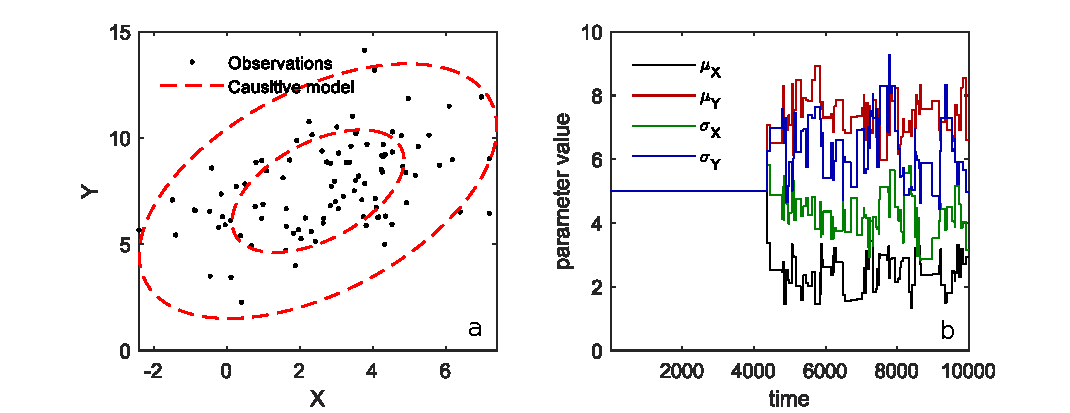
\includegraphics[scale=0.75]{init-problems.pdf}
	\caption{(a) Observed data from the underlying causitive model, whose parameters will be the inference target. (b) First 10 000 iterations of an ABC-MCMC scheme with a uniform kernel. The algorithm initially struggles to find a region of non-zero probability from a random starting position within the parameter space.}
	\label{init-qualms}
\end{figure}

%Figure of the chain becoming stuck at the beggining

While ABC-MCMC and the uniform weighting kernel $K_U$ offers improved acceptance rates compared to a rejection scheme, it is not without faults. Firstly, it can suffer from an initialisation problem, as highlighted in figure \ref{init-qualms}(b). Compounding this, the acceptance rate can rapidly decline past a certain threshold as tolerance is decreased. This is a syptom of the same problem as initialisation. Each move is either flat out rejected or is determined to be part of the posterior. This makes it prone to becoming stuck when in the tails of a distribution. This is especially problematic in high-dimensional search spaces where the posterior density is an extraordinarily small volume. Ideally, if in a poor spot, the algorithm should be able to make local transitions toward an area of high probability density. However, this adjustment will involve abandoning the $K_U$. A weighting kernel which offers infinite support is needed. That is, the weight dimishes with distance, however it never reaches zero. Fortunately many functions have the required properties. In this text we favour a  weighting kernel based on the Gaussian distribution, $K_G$. This choice is advantageous as the log-distance can be evaluated for stable computation in sampling algorithms. This implementation mirrors the stable implementation of likelihood values, expanded upon in \hyperref[AppendixB]{Appendix B}.\\

For an observed dataset $\bm{S}(\bm{y})$ and simulated dataset $\bm{S}(\bm{y^*})$, where $\bm{S} = \{S_1,\dots,S_O\}$, the weighting kernel would be computed as:
\begin{equation}
p(\bm{S}(\bm{y})|\bm{S}(\bm{y^*}),\bm{\theta}) = K_G\big(\text{d}(\bm{S}(\bm{y}),\bm{S}(\bm{y^*}))\big) \propto \prod_{i = 1}^{O} \text{exp}\Big[-\frac{1}{2}\Big(\frac{\text{d}(S_i(\bm{y}),S_i(\bm{y^*}))}{\epsilon_i}\Big)^2\Big]
\end{equation}
Figure \ref{KuVSKg-1} compares and contrasts $K_U$ and $K_G$ over the first 7 500 time steps in an ABC-MCMC algorithm targeting the parameters to a bivariate Gaussian distribution, $\bm{\theta} = \begin{bmatrix}
\bm{\mu}\ \bm{\Sigma}
\end{bmatrix}$. $K_G$ does not suffer from the same initialisation problem as $K_U$. $K_G$ also has an improved accpetance rate and better mixing when compared to $K_U$. Figure \ref{KuVSKg-2} demonstrates that with time both kernels converge to the same solution.\\

Both figure \ref{KuVSKg-1} and \ref{KuVSKg-2} show an insensitivity to $\rho$. This is a direct result of the insufficiency of the selected summary statistics for that parameter. This reinforces that while a smaller $\epsilon$ improves $\pi(\bm{\theta}|\text{d}(S(\bm{y}),S(\bm{y^*}))<\epsilon) \approx \pi(\bm{\theta}|S(\bm{y}))$, but if the summary statistics are not informative such that $\pi(\bm{\theta}|S(\bm{y})) \approx \pi(\bm{\theta}|\bm{y})$, then the house of cards falls apart. In this case the statistic $\text{cov}(X,Y)$ which should be sensitive to $\rho$, remains overwhelmed by $\sigma_X$ and $\sigma_Y$. In this case, the sample correlation, $\bar{\rho}$, may have been a better summary statistic choice. 

\begin{figure}[H]
	\centering
	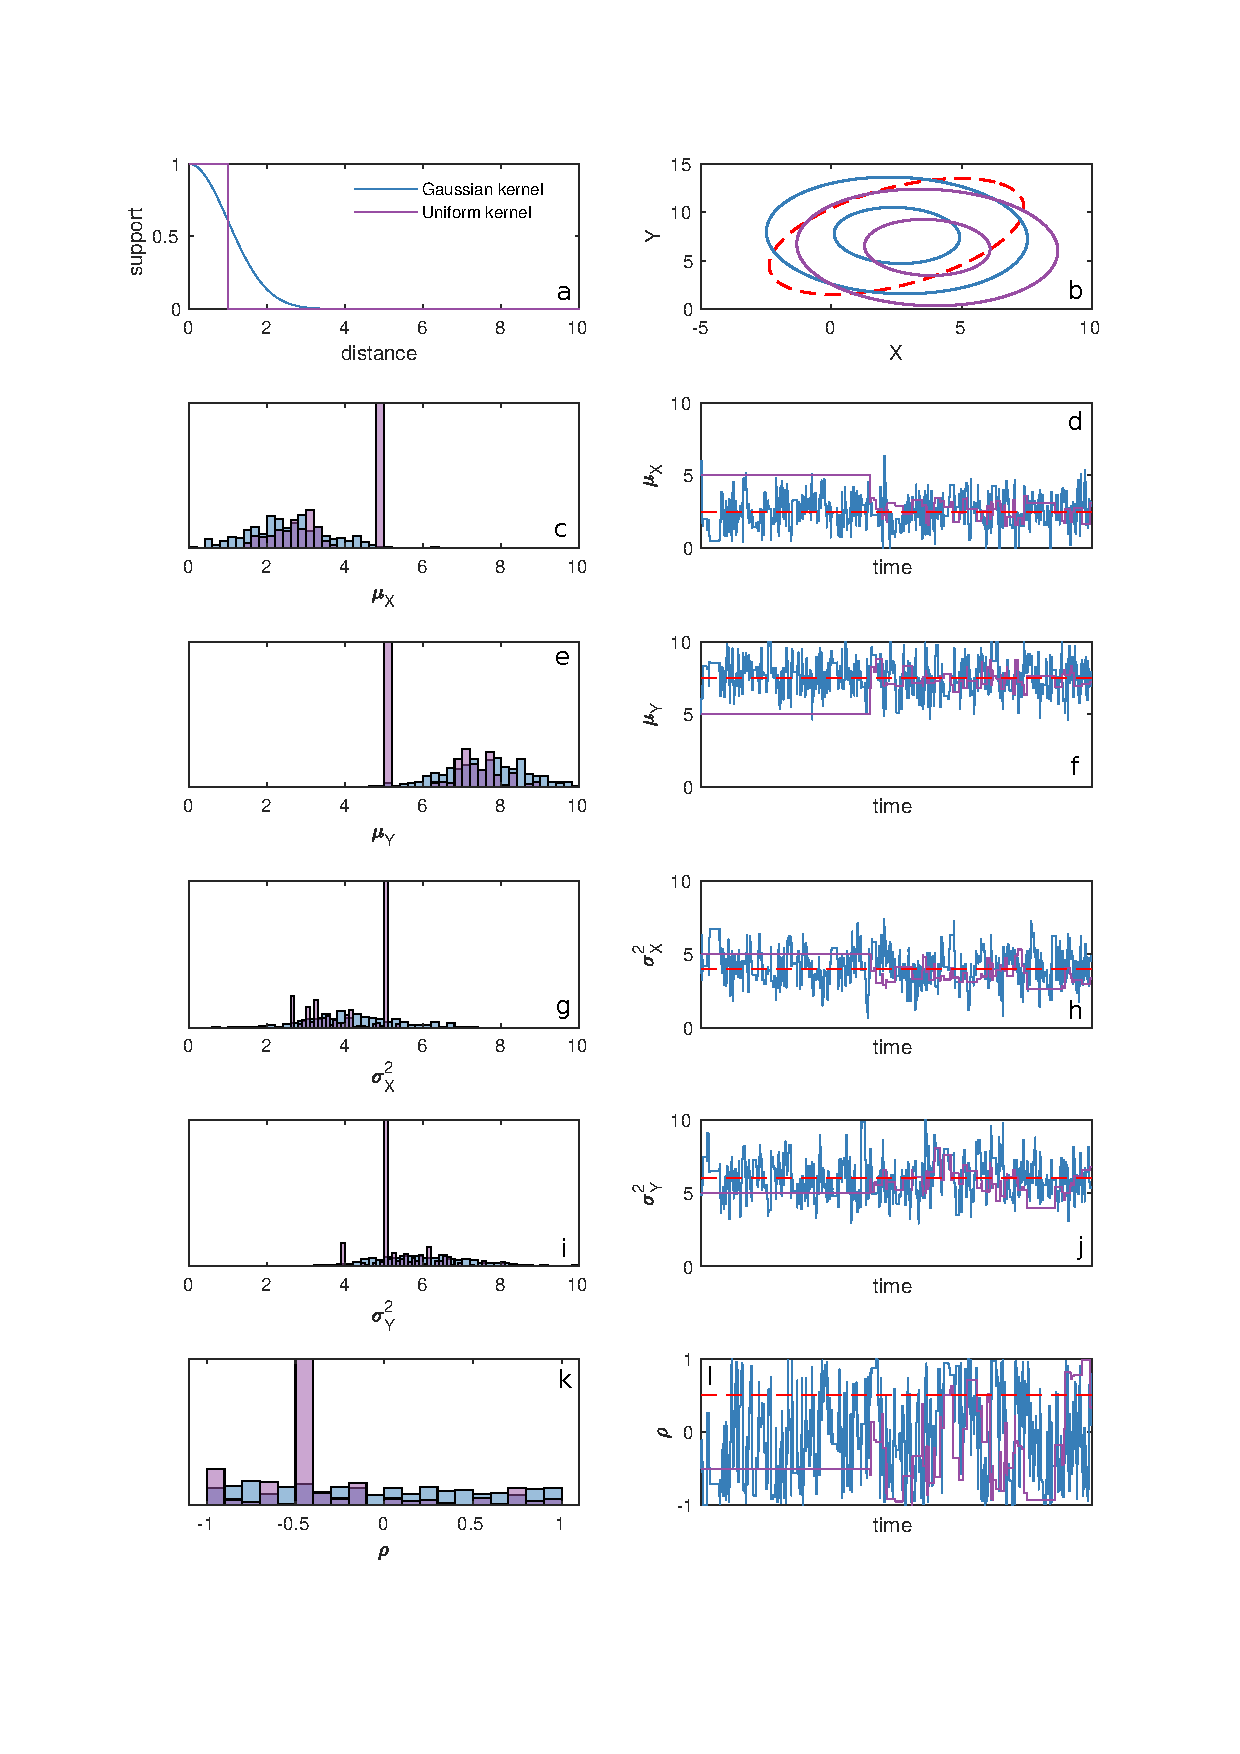
\includegraphics[scale=0.8]{BG10000.pdf}
	\caption{To-Do: Add caption}
	\label{KuVSKg-1}
\end{figure}

\begin{figure}[H]
	\centering
	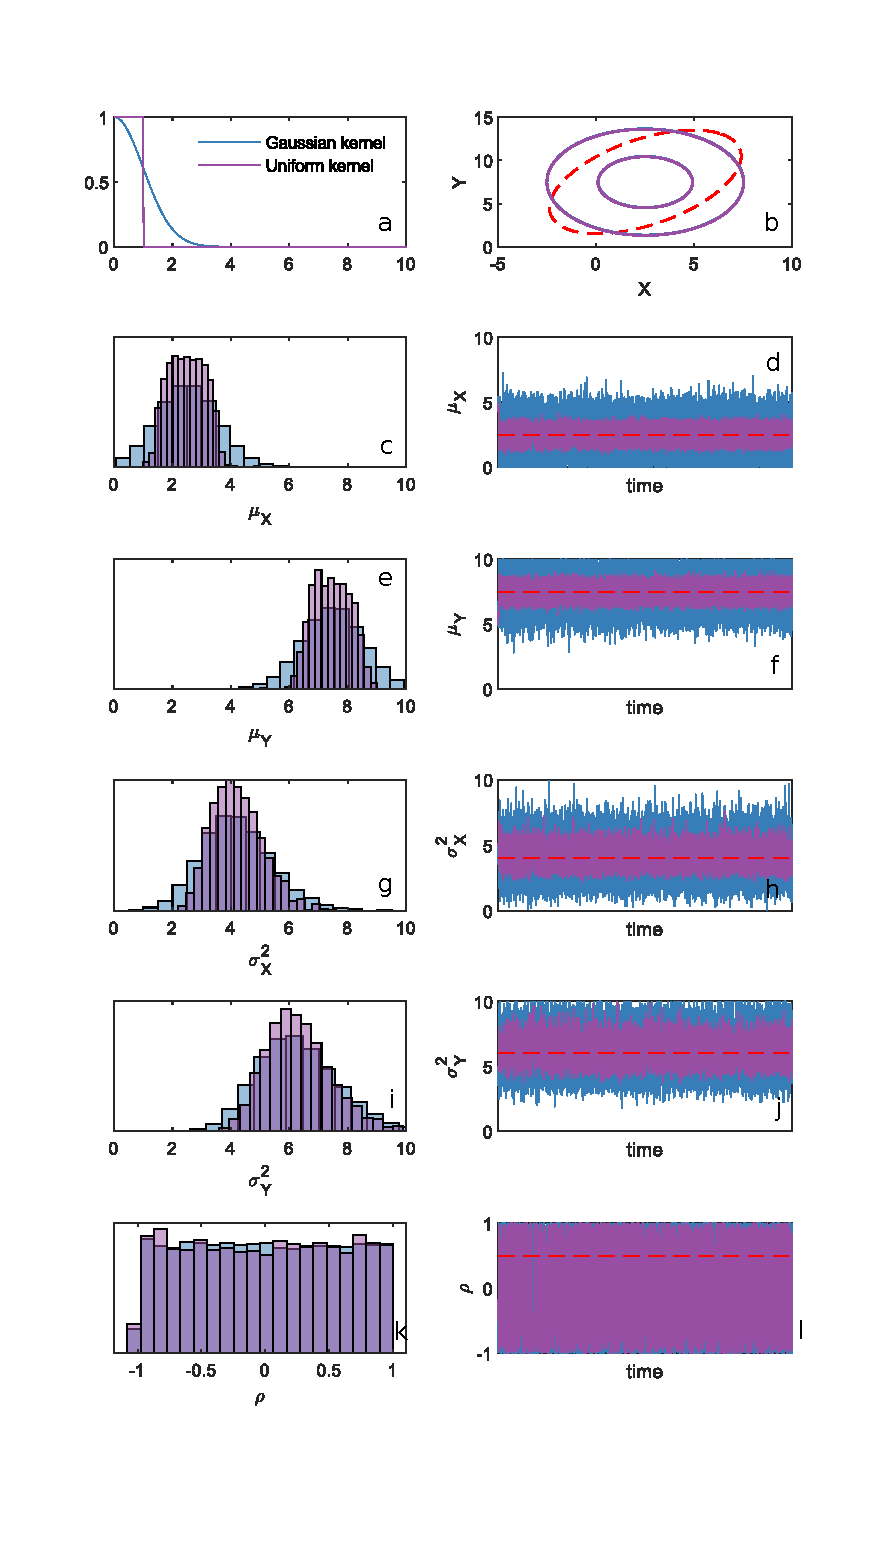
\includegraphics[scale=0.8]{BG1000000.pdf}
	\caption{To-Do: Add caption}
	\label{KuVSKg-2}
\end{figure} 

\section{Toy problem 4: Banana distribution}

As a fourth example we desgin a more challenging problem, one for which there are no imediate and obvious summary statistics and has some degree of dimensionality. Consider we have $n = 1000$ observations from a "banana" distribution, Figure \ref{banana-data}. To define the banana distribution, we start with a 2-dimensional Gaussian distribution:
\begin{equation}
\begin{bmatrix}
x\ y
\end{bmatrix}=\mathcal{N}(\bm{\mu},\bm{\Sigma}),\ \bm{\mu} = \begin{bmatrix}
\mu_X\ \mu_Y
\end{bmatrix}^T,\ \bm{\Sigma} = \begin{bmatrix}
\sigma^2_X & \rho\sigma_X\sigma_Y\\
\rho\sigma_X\sigma_Y & \sigma^2_Y
\end{bmatrix} 
\label{gauss-banana}
\end{equation}
The Gaussian co-ordinates $x$ and $y$ are then twisted to produce a more nonlinear target, $X$ and $Y$, using:
\begin{equation}
X = b_1x
\label{x-banana}
\end{equation}
\begin{equation}
Y = y/a-b_2(b_1^2x^2+b_1^2)
\label{y-banana}
\end{equation}
In total the parameters which define this model are $\bm{\mu}$, $\bm{\Sigma}$ and the banana parameters $\begin{bmatrix}
b_1\ b_2
\end{bmatrix}$. Here the unknown target parameters are $\bm{\mu} = \begin{bmatrix}
0\ 0
\end{bmatrix}^T$,
$\bm{\Sigma} = \begin{bmatrix}
\sigma^2_X & \rho\sigma_X\sigma_Y\\
\rho\sigma_X\sigma_Y & \sigma^2_Y
\end{bmatrix}$ while $\begin{bmatrix}
b_1\ b_2
\end{bmatrix}$ = $\begin{bmatrix}
1\ 1
\end{bmatrix}$. 

\begin{figure}[H]
\centering
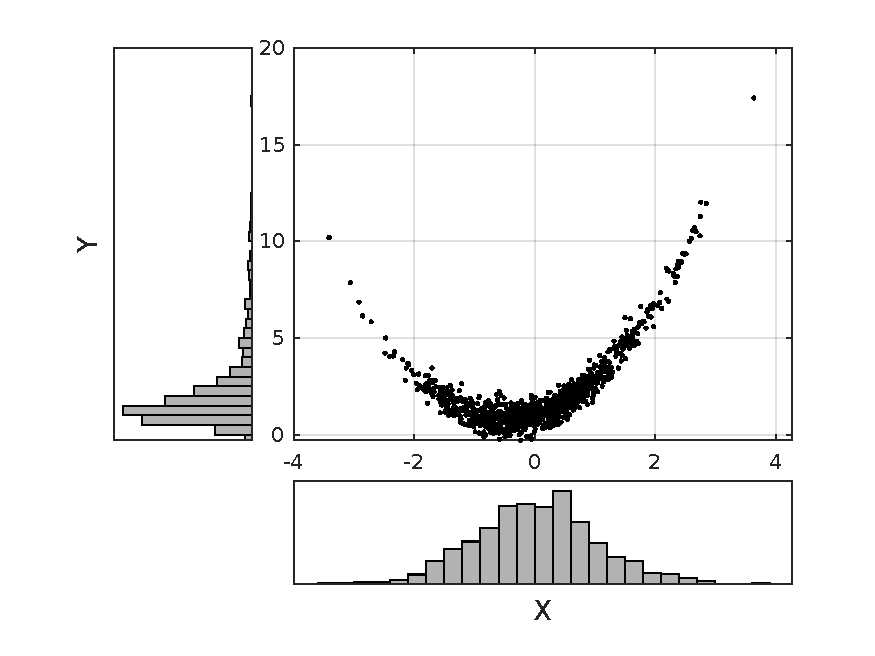
\includegraphics[scale=1]{banana-data.pdf}
\caption{$n = 1000$ observations from the "banana" distribution, analytically defined by equations \ref{gauss-banana}, \ref{x-banana}, \ref{y-banana}. 
This problem is more challenging as there is no immediately apparent sufficient statistics to facilite ABC estimation of the unknown parameters.}
\label{banana-data}
\end{figure}

To proceed with ABC inference under this model we must define a set of reasonably sufficient statistics. In the previous examples it has been possible to use the sample values for each of the unknown parameters, however, here this proved to be insufficient in a trial run. In the ABC literature summary statistic selection is the focus of technique development and active research. \citet{Blum2013} and \citet{Prangle2017} offer reveiws of this research area. For this example we heed the advice of \citet{Wood2010}. Firstly, the statsitics have the same role in ABC as the data do in a traditional likelihood. Hence, there is no need for certain statistics to relate to specific parameters any more than there is the need for certain data points to relate to specific parameters. The key is in indenitifying a set of statistics which is senstitive to the scientificaly important and repeatable features of the data, and insensitive to the transient noisey components. \citet{Wood2010} identifies marginal distribution statistics as being a useful first step. The marginal distribution for our banana observations, $X$ and $Y$, are plotted in figure \ref{banana-data}. Here we can see $X$ appears as a regular Gaussian distribution, while $Y$ appears as a skewed-Gaussian distribution. This motivates the choice of marginal statistics for $X$ as the sample mean, $\bar{\mu_X}$, and sample standard deviation, $\bar{\sigma_X}$. While marginal statistics for $Y$ are sample skewness $\bar{\gamma_Y}$, as well as $\bar{\mu_Y}$ and $\bar{\sigma_Y}$. However, this does not capture the "shape" of the joint distribution in 2D dimensions. To capture the bananity of the joint distribution we fit a second degree polynomial to the data, $Y = aX^2 + bX + c$. The co-effecient values $a$, $b$ and $c$ are then used as the summary statistics. For this example we consider this set, $\begin{bmatrix}
\bar{\mu_X}\ \bar{\sigma_X}\ \bar{\gamma_Y}\ \bar{\mu_Y}\ \bar{\sigma_Y}\ a\ b\ c
\end{bmatrix}^T$, to constitute reasonably sufficent summary statistics for the banana distribution. However, these are not perfect, and the effect of using them will be the introduction of some degree of bias into the posterior. \\



% Introduce scaling considerations
In our applications so far the distance metric has been a vector composed of the absolute distance between observed and simulated summary statistics, hence:
\begin{equation}
\text{d}_i(S_i(\bm{y}),S_i(\bm{y^*})) = |S_i(\bm{y})-S_i(\bm{y^*})|
\end{equation}
is the marginal fit for a given statistic. In our examples it has not been necessary to consider the scale the chosen statistics vary over and their sensitivity to the unknown parameters. For the most part all statistics have been equally sensitive and varied over a similar scale. Under a rejection scheme where all simulations and distances can be computed before the rejection step, it is straight forward to normalize the distances by the scale they vary over. However, it is not clear how to best account for this scale and sensitivity when using ABC-MCMC. One solution would be to use variable tolerances which account for this scale and sensitivity, establishing $\epsilon = \{\epsilon_1,\dots,\epsilon_O$. However, this is not a user friendly solution to the issue of scale as implementation would invariably involve many repitions as $\epsilon$ is tuned. Other authors, citet{Ratmann2010}, have normalised the marginal weighting term, the weight for each individual statistic, to one. I attempt a transformation in a similar spirit by approximating a term $\sigma_{S_i}$ which will normalize the distance for each statistic to one. In algorithms distance is replaced by a normalized-distance:
\begin{equation}
\hat{d_i}(S_i(\bm{y}),S_i(\bm{y^*})) =  \frac{|S_i(\bm{y})-S_i(\bm{y^*})|}{\sigma_{S_i}}
\end{equation}

% Computing the normalization term
A good sampling algorithm would temper $\bm{\sigma_S} = \{\sigma_{S_1},\dots,\sigma{S_O}$ on the fly. Without such an algorithm $\bm{\sigma_S}$ must be predefined. Here we favour a Monte Carlo approximation based on $k > 10\ 000$ simulations from the prior and given the observed data. A marginal term $\sigma_{S_i}$ is then defined as the sample standard deviation of the distance between the simulated summary statistic and the observed summary statistic:
\begin{equation}
\sigma_{S_i} = \sqrt{\frac{\sum_{i = 1}^{k}(\text{d}_i)^2}{k-1}}
\end{equation}
This does not preclude varying $\epsilon$, however, it does ensure that each marginal $\epsilon_i$ is of a simular magnitude. \\



Figure \ref{MH-banana} shows the results of an ABC-MCMC algorithm targeting the banana distribution. This leverages a Gaussian kernel, summary statistics as described and uses a normalized distance metric. For this problem only the Gaussian parameters, $\bm{\mu}$ and $\bm{\Sigma}$ are unknown.\\

% Insert banana problem solved w/ MCMC + MLE plot
\begin{figure}[H]
	\centering
	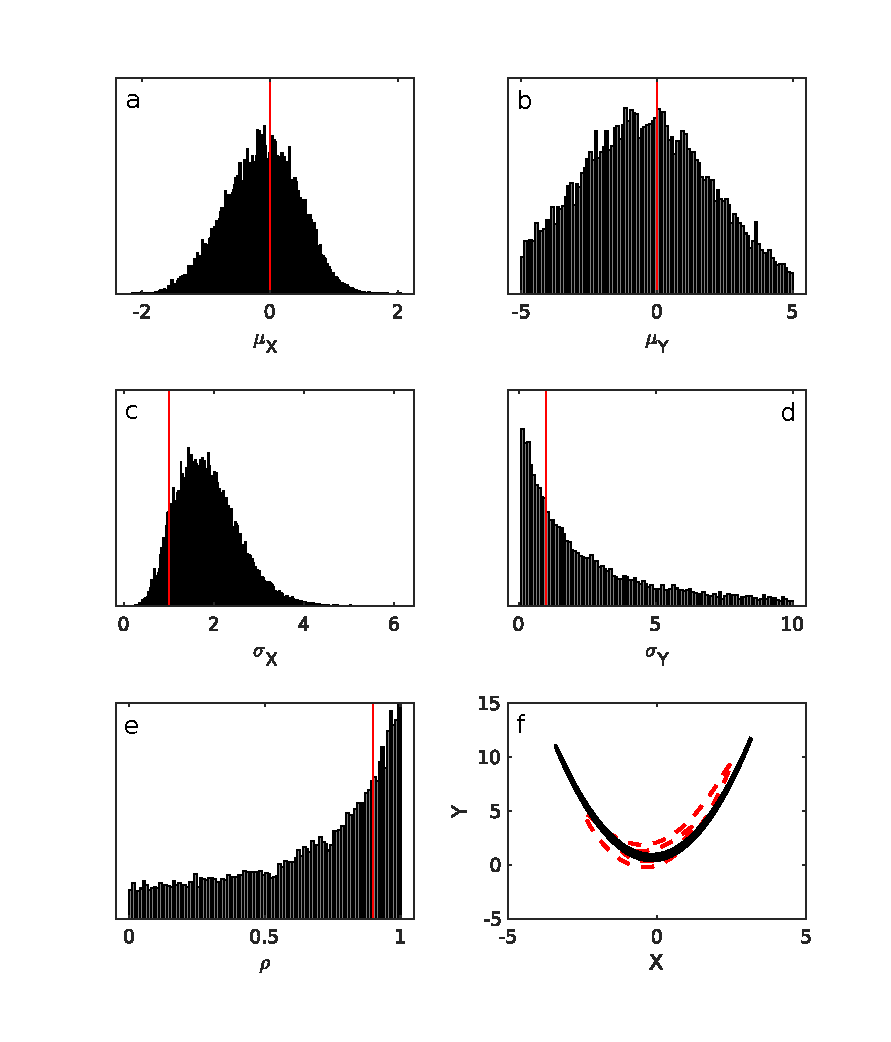
\includegraphics[scale=1]{MH-Banana-1mil.pdf}
	\caption{The marginal posterior distributions for banana parameter inference, as well as the median posterior model (f), in black, compared to the original model, red dashed lines. Red lines mark the true parameter values on the marginal posterior plots. I justify the legitimacy of extracting the median marginal model as there are limited correlations between the unknown parameters.}
	\label{MH-banana}
\end{figure}

Throughout this chapter, I plot the median marginal posterior model. That is, the model which is defined by taking the median of the Markov chain for each individual parameter. One example is figure \ref{MH-banana}(f), here the red dashed lines mark the 50\% and 95\% confidence intervals of the model the data was generated from, while the solid black lines mark the 50\% and 95\% confidence intervals of the median marginal posterior model. Often the marginal parameter densities are considered as the principal result from Bayesian parameter inference. However, the marginal posterior distributions hide correlations between parameter which may be present in the joint posterior, which is the distribution the Markov chain sampled. If there are correlations between parameters then a given parameters uncertainty will appear greater in the marginal distribution. To keep inference honest I plot the correlations between each parameter, figure \ref{correlation-plot}, from the Markov chain generated by \ref{MH-banana}. As can be seen there are limited correlations between parameters. As a result extracting the marginal median is an accurate representation of the median model under the joint distribtuion. An accurate estimate of the uncertainty can also be found by taking the marginal standard deviation. If there was significant uncertainty between some $\theta_1$ and $\theta_2$ then it would not make sense to evaluate $\theta_2$ marginally with $\theta_2 = \mu \pm \sigma$. Instead $\sigma$ would need to be evaluated with respect to a given value for $\theta_1$, in order to have a proper understanding of the uncertainty in $\theta_2$. 

% Insert correlation plot of 5 pars to justify taking the MLE
\begin{figure}[H]
	\centering
	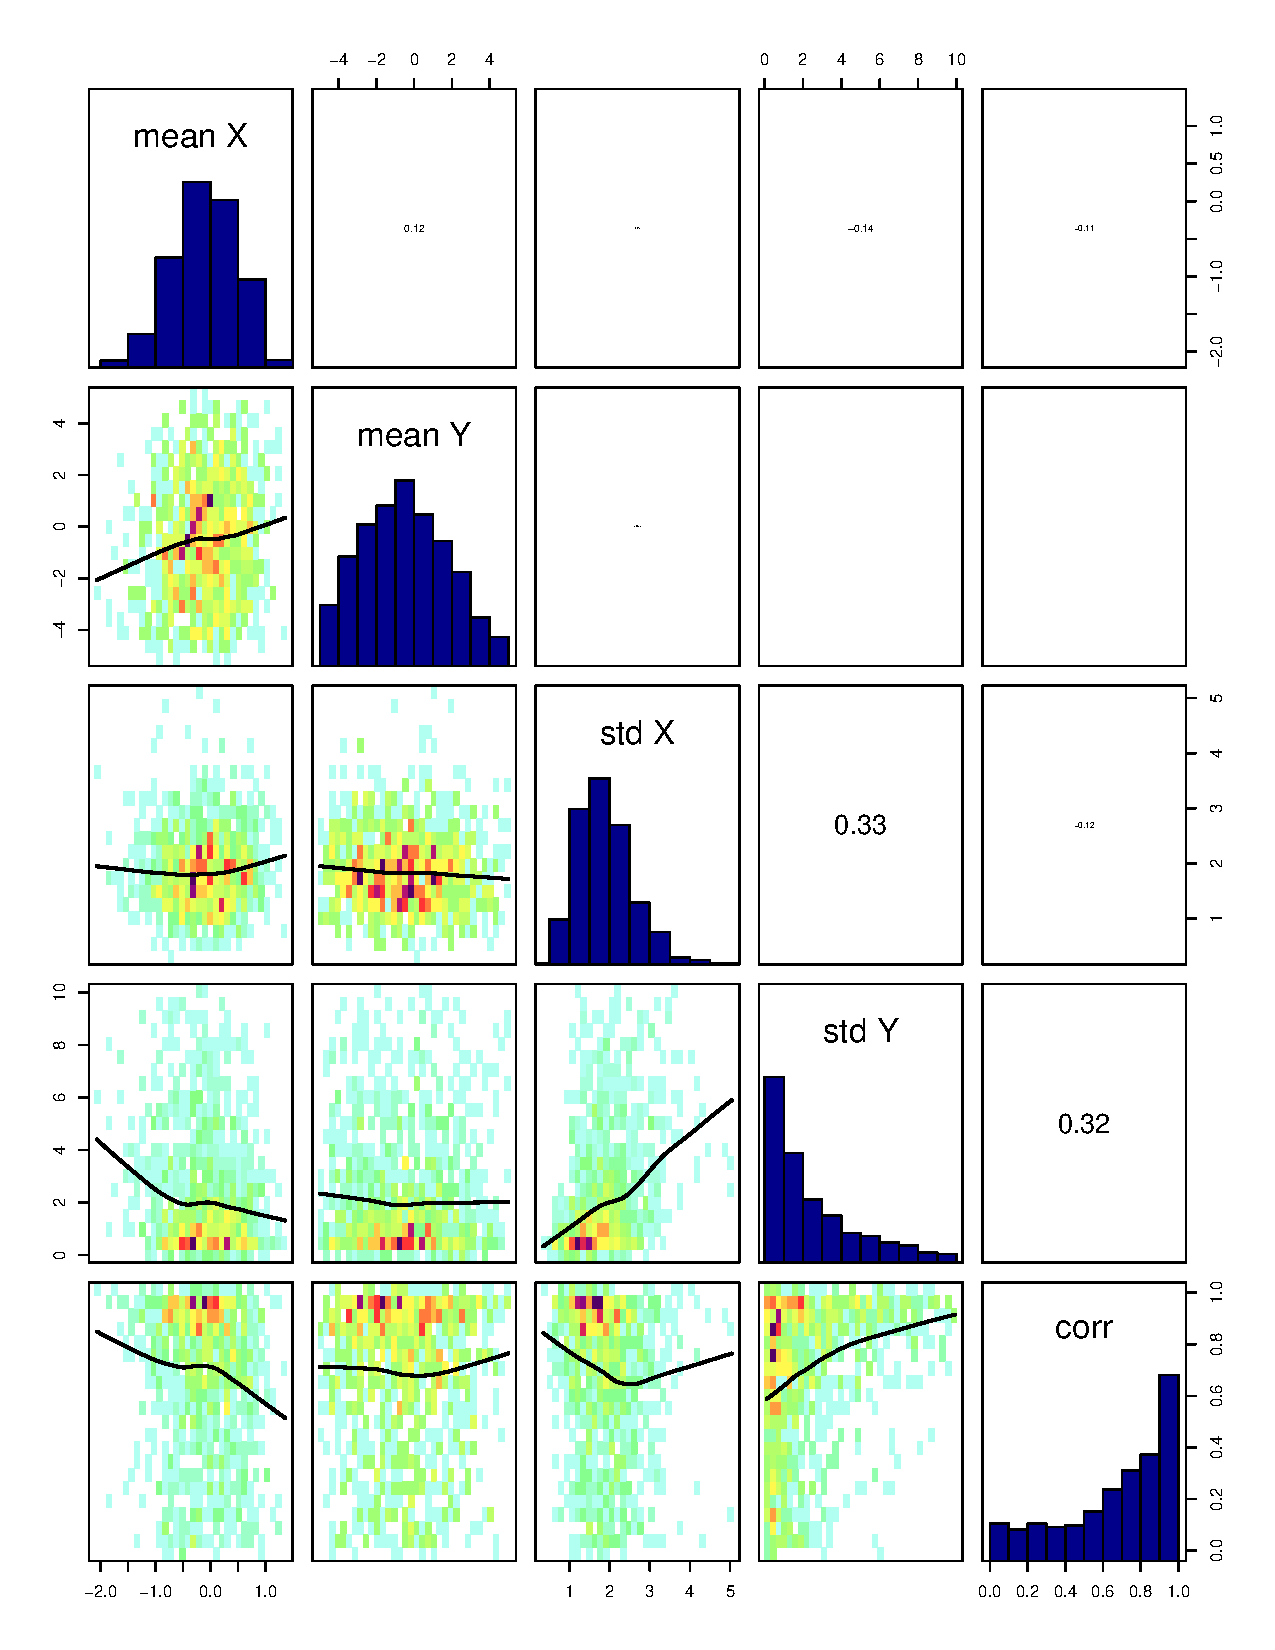
\includegraphics[scale=0.6]{correlation-plot.pdf}
	\caption{Correlation plot for the Markov chain in figure \ref{MH-banana}. There is limited correlation between the parameters. This is used as justification for plotting statistics of the marginal posterior as representative of the joint posterior.}
	\label{correlation-plot}
\end{figure}


The performance of our MCMC algorithm as described by algorithm \ref{ABC-MCMC} depends on the users ability to choose a suitable proposal distribution $q(.,.)$. If we limit ourselves to a multivariate Gaussian distribution, then we must choose a suitable covariance matrix. If the variance for each parameter is too large then the probability of accepting a proposal will be low, as each step will be erratic and far from the current location. Consider that as the variance for $q(.,.) \rightarrow \infty$ we effectively have a Monte Carlo scheme. However, if the variance is too small then the acceptance rate will be very good but algorithm will fail to explore the full parameter space. Hence there is a balance encoded in the selection of the proposal distribution. We desire both a reasonable acceptance and a good exploration of the parameter space. In this way we select a proposal distribution which suits the underlying target distribution. Generally it is simplest to leave the off-diagonal terms in the proposal distribution, the correlations between parameters, unconsidered.\\

However, such a system is not ideal. Selecting an optimal proposal distribution is non-trivial problem. Here we can turn to theoretical developments to guide a better proposal distribution. \citet{gelman1996} show that when the target distribution is Gaussian, an efficient sampler can be constructed by scaling the proposal covariance to $2.4^2/d$, where $d$ is the number of unknown parameters. In th previous sections it has been best to ignore the correlations between parameters. However, these correlations can be important to consider, if there are strong parameter correlations in the posterior then sampling success can be weakened by leaving these set to 0, especially in a high dimensional space and for nonlinear problems. But knowing about these correlations and designing a pre-defined proposal is next to impossible. Ideally the algorithm should be able to learn about the posterior on the fly, and if there are correlations betweeen parameters, adjust accordingly. With this in mind \citet{haario2001} developed Adaptive Metropolis (AM). AM tunes the proposal distribution to the posterior distribution by using the history of the chain generated so far. After some designated time, $t$, the covariance matrix of the proposal distribution, $\bm{\Sigma_q}$, is set to the covariance of the Markov chain so far. 
\begin{equation}
\bm{\Sigma_q} = \text{cov}(\bm{\theta}_1,\dots,\bm{\theta}_t)s_{AM} + I\upsilon
\end{equation}
Where $s_{AM}$ is the scaling factor, generally $2.4^2/d$, and $\upsilon$ is a small positive which prevents the covariance from becoming singular. AM is compared to MH in table \ref{sampling-method-comparison}.\\

Figure \ref{AM-demonstration} plots the effect AM has on a sub-optimal choice for a proposal distribution, and the computational advantage gained from adaption. \\

\begin{figure}[H]
	\centering
	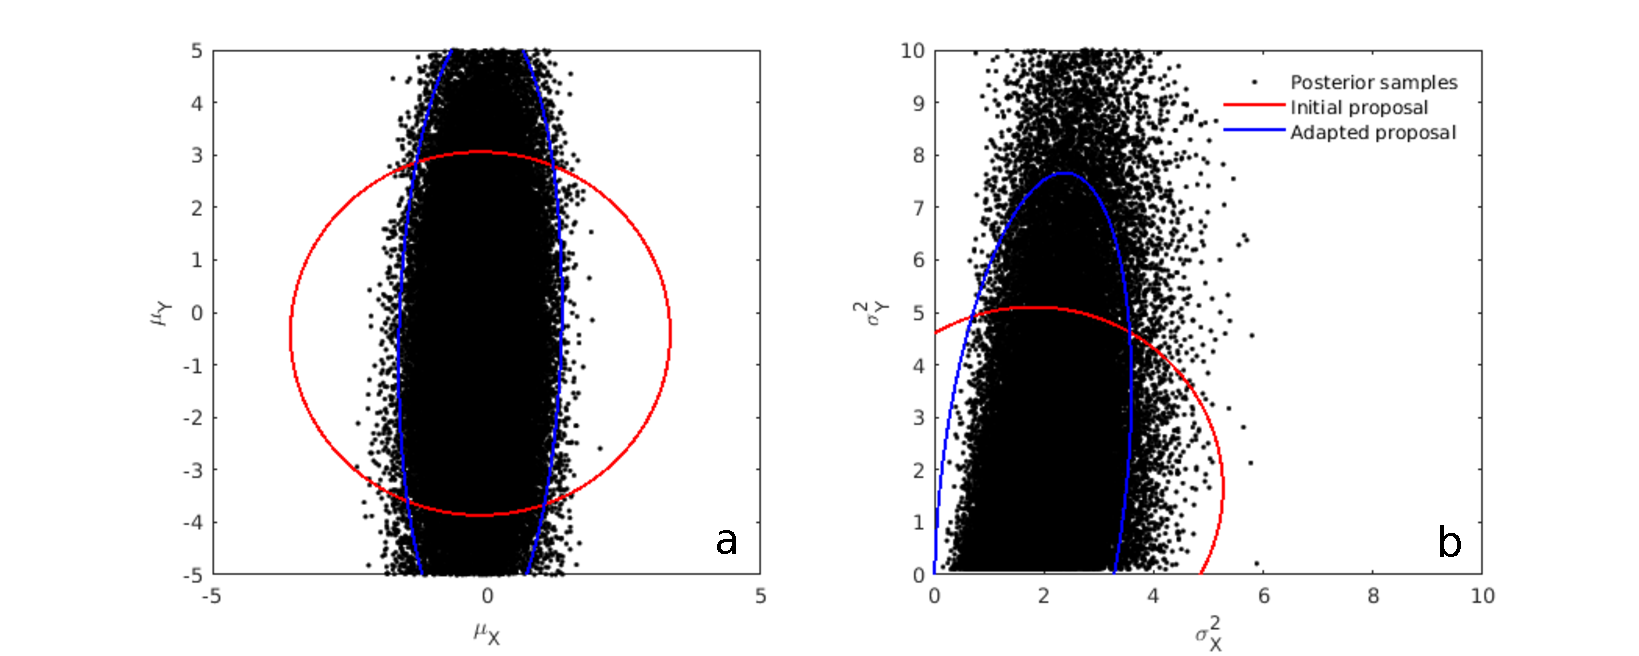
\includegraphics[scale=0.7]{Am-demonstration.pdf}
	\caption{Adaptive proposal distribution compared to a suboptimal proposal which was the basis of the MCMC algorithm in figure \ref{MH-banana}.}
	\label{AM-demonstration}
\end{figure}

Delayed Rejection (DR) can also be implmented to improve sampling efficiency \citet{Mira2001}. Under DR, when a proposed move is rejected, instead of advancing a time step and retaining the same position, another proposed candidate move is considered. The acceptance probability of the second proposal differs from the M-H acceptance probability in order to retain time reversibility of the Markov chain, ensuring that the chain converges to the desired stationary distribution. When a Markov chain remains in the position over time, the estimates obtained by averaging along the chain become less efficient. Increases to autocorrelation of the chain increase the variance of estimates based on the chain \citep{Mira2001}. In this way DR is more effecient than a standard MH algorithm. A two-stage DR algorithm, as is considered in implementations here, would operate as follows. \\

At the first stage the acceptance probability is the Metroplis-Hastings acceptance probability:
\begin{equation}
	\alpha_1(\theta,\theta^*) = \text{min}\bigg\{1,\frac{\pi(\theta^*)q_1(\theta^*,\theta)}{\pi(\theta)q_1(\theta,\theta^*)} \bigg\}
\end{equation}
where $\pi$ is the target distribution of the algorithm and $q_1$ is the proposal distribution. If the proposed move to $\theta^*$ is rejected then a second candidate move, $\theta^{**}$, can be considered from the second proposal distribution $q_2$. The acceptance probability for $\theta^{**}$ is:
\begin{equation}
	\alpha_2(\theta,\theta^*,\theta^{**}) = \text{min}\bigg\{1,\frac{\pi(\theta^{**})q_1(\theta^{**},\theta)q_2(\theta^{**},\theta^*,\theta)[1-\alpha_1(\theta^{**},\theta^*)]}{\pi(\theta)q_1(\theta,\theta^*)q_2(\theta,\theta^*,\theta^{**})[1-\alpha_1(\theta,\theta^*)]} \bigg\}
\end{equation}
Here I limit implementation to a two-stage DR scheme and use a $q_2$ with a smaller covariance matrix. $q_1$ is downscaled to give $q_2$ by the relation, $q_2 = q_2/s_{DR}$. DR is compared to MH and AM in table \ref{sampling-method-comparison}.\\

Both Adaptive Metropolis and Delayed Rejection can be implemented together to give a Delayed Rejection Adaptove Metropolis scheme, as was first implemented by \citet{Laine2008}. There are many implementation possibilities given the mixing of AM and DR. Here a straight forward implementation is favoured, as in \citet{Laine2008}, which retains the principal advantages of each method to give an efficient adaptive algorithm.    The first stage proposal is adapted to the chain generated so far, and one scaled down second stage proposal is considered. The second stage proposal inherits the adapted covariance matrix of the first stage proposal, only the variance is down scaled. DRAM is compared to MH, AM and DR in table \ref{sampling-method-comparison}.\\

When running a 'one-size fits all' generic MCMC algorithm, the standard procedure is to propose a candidate move which updates each and every parameter value. If we are at the position $\bm{\theta_{i-1}}$ in the parameter space, then the proposal distribution suggests a candidate move:
\begin{equation}
	\bm{\theta_{i}} = \mathcal{N}(\bm{\theta_{i-1}},\bm{\Sigma_q})
\end{equation}
However, this is not the only option. Another generic choice is to update a single parameter per time step. Much like the variance of $\bm{\Sigma_q}$, there is a trade-off between acceptance rate and speed of parameter space exploration encoded into this decision. Table \ref{sampling-method-comparison} compares the acceptance rate of a MH algorithm where all parameters are updated at once, and an MH algorithm where a single parameter is updated per time step. A significant increase in acceptance rate is made through this change. There is also a third option. At each time step a sub-set of parameters are updated. This is referred to as blocking. When parameters that are correlated are updated as block together, sampler performance is increased relative to updating each dimension independantly \citep{Turek2017}. However, implementing effective parameter blocking is not user friendly and requires problem specific implementation. 

\begin{table}[H]
	\centering
	\begin{tabular}{|c|c|}
	\hline
	Sampling method & Acceptance rate (\%) \\
	\hline
	Metropolis-Hastings (MH) & 5.22\% \\
	\hline
	Adaptive Metropolis (AM) & 10.63\% \\
	\hline
	Delayed Rejection (DR) & 28.35\% \\
	\hline
	Delayed Rejection Adaptive Metropolis (DRAM) & 36.44\% \\
	\hline
	Single parameter update & 35.83\% \\
	\hline
	\end{tabular}
	\caption{My first table}
	\label{sampling-method-comparison}
\end{table}



\begin{figure}[H]
\centering
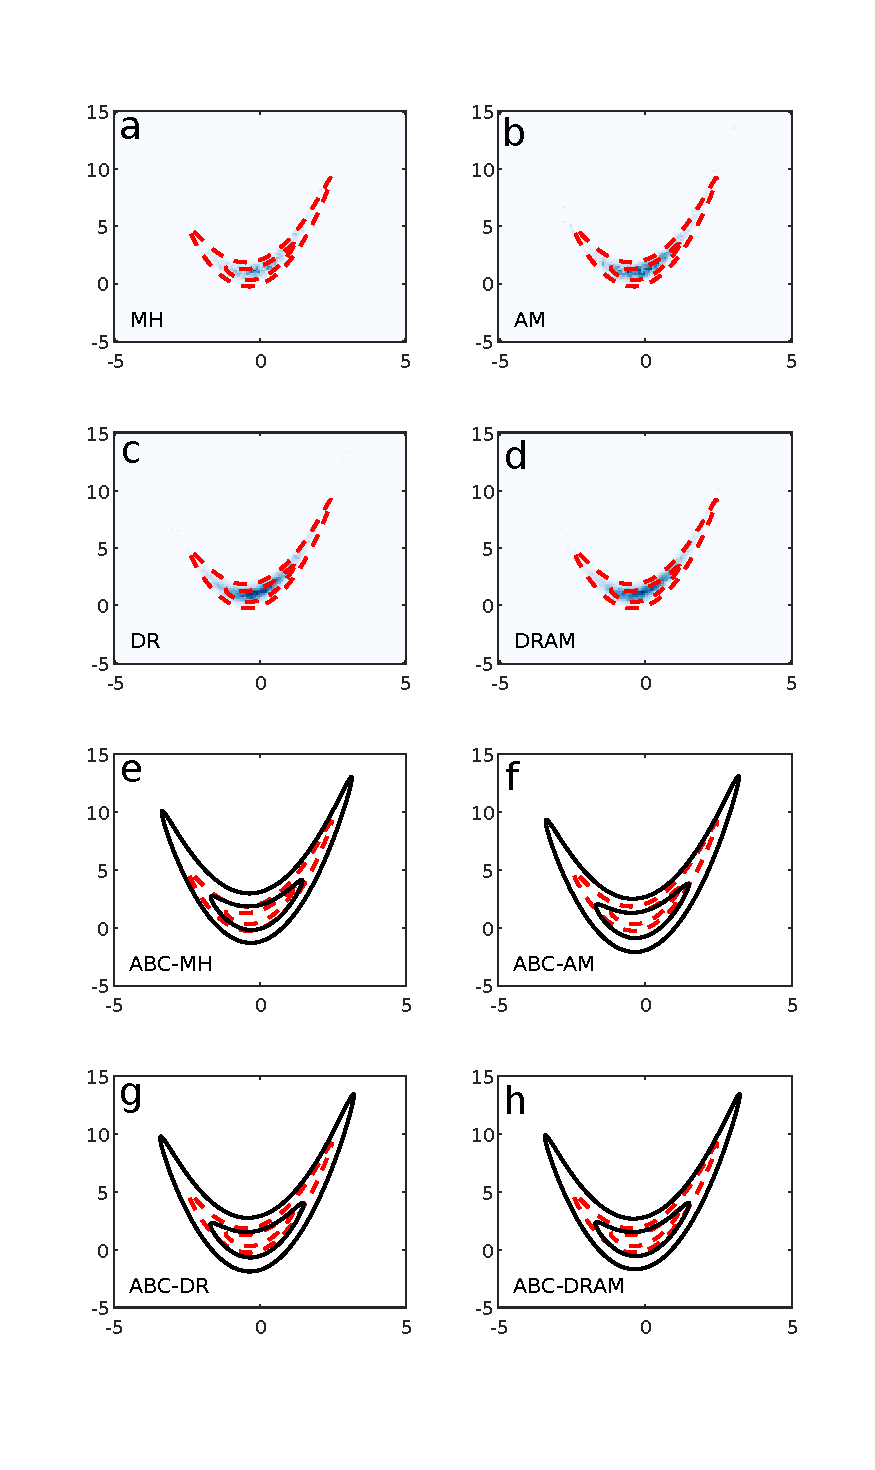
\includegraphics[scale=0.9]{BananaABCvsMCMC.pdf}
\caption{Pdf test}
\end{figure}

\begin{figure}[H]
\centering
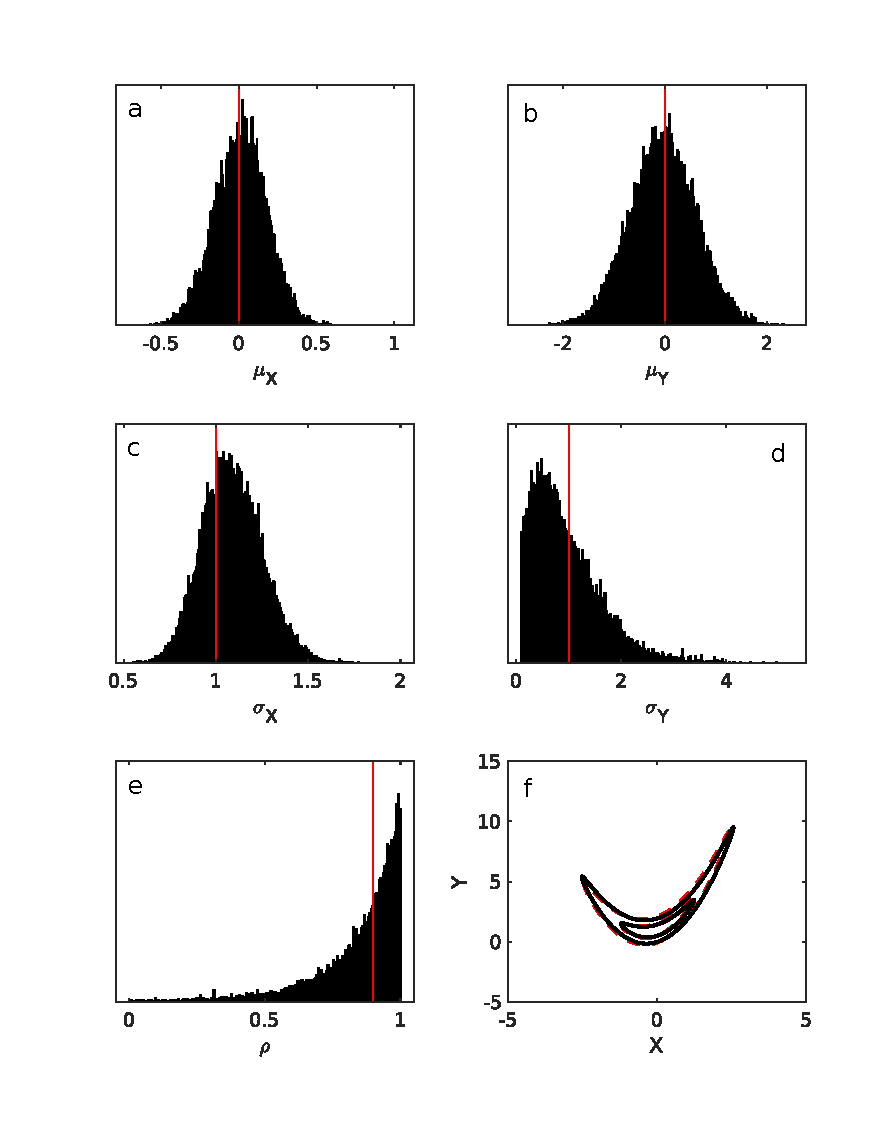
\includegraphics[scale=1.1]{DRAM-blocked-banana.pdf}
\caption{Best banana}
\end{figure}